\section{harps::CurrentTime Class Reference}
\label{classharps_1_1CurrentTime}\index{harps::CurrentTime@{harps::CurrentTime}}
{\tt \#include $<$clock.hpp$>$}

Inheritance diagram for harps::CurrentTime::\begin{figure}[H]
\begin{center}
\leavevmode
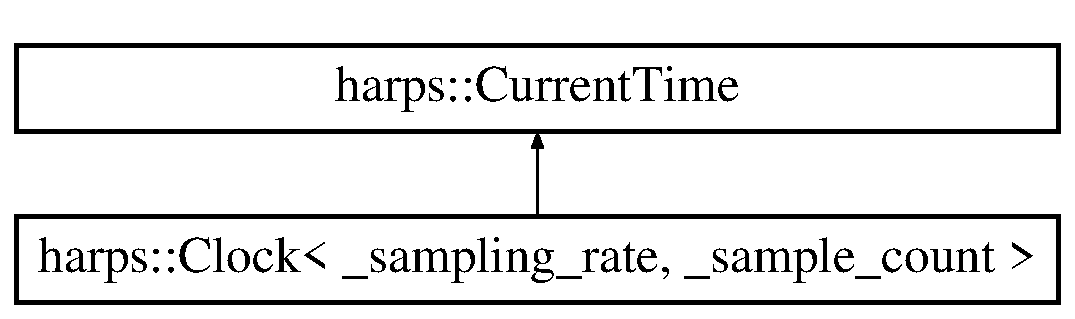
\includegraphics[height=2cm]{classharps_1_1CurrentTime}
\end{center}
\end{figure}
\subsection*{Public Types}
\begin{CompactItemize}
\item 
enum \{ \textbf{MATRIX\_\-COUNT} =  3
 \}
\end{CompactItemize}
\subsection*{Public Member Functions}
\begin{CompactItemize}
\item 
{\bf CurrentTime} (Time \_\-tick\_\-length)
\item 
virtual {\bf $\sim$CurrentTime} ()
\item 
{\footnotesize template$<$unsigned int \_\-which$>$ }\\double {\bf getTime} (unsigned int \_\-offset) const 
\item 
void {\bf reset} ()
\item 
{\footnotesize template$<$unsigned int \_\-which$>$ }\\void {\bf swapMatrix} (TimeMatrix \&\_\-matrix)
\item 
{\footnotesize template$<$unsigned int \_\-which$>$ }\\const TimeMatrix \& {\bf getMatrix} () const 
\item 
void {\bf noteOn} (int \_\-note)
\item 
void {\bf noteOff} ()
\item 
void {\bf setPitchBend} (float \_\-pitch)
\item 
float {\bf getToneFrequency} () const 
\item 
int {\bf getTone} () const 
\item 
float {\bf getPitchBend} () const 
\item 
void {\bf tick} (unsigned int \_\-sample\_\-count)
\end{CompactItemize}


\subsection{Detailed Description}
現在時刻を保持します。現在時刻は4つの時刻変換行列を通して取得することができます。 

\subsection{Constructor \& Destructor Documentation}
\index{harps::CurrentTime@{harps::CurrentTime}!CurrentTime@{CurrentTime}}
\index{CurrentTime@{CurrentTime}!harps::CurrentTime@{harps::CurrentTime}}
\subsubsection[CurrentTime]{\setlength{\rightskip}{0pt plus 5cm}harps::CurrentTime::CurrentTime (Time {\em \_\-tick\_\-length})\hspace{0.3cm}{\tt  [inline]}}\label{classharps_1_1CurrentTime_6a58e37c3b82280888f7d39e9387fda9}


コンストラクタ \begin{Desc}
\item[Parameters:]
\begin{description}
\item[{\em \_\-tick\_\-lenght}]1クロックの時間 \end{description}
\end{Desc}
\index{harps::CurrentTime@{harps::CurrentTime}!$\sim$CurrentTime@{$\sim$CurrentTime}}
\index{$\sim$CurrentTime@{$\sim$CurrentTime}!harps::CurrentTime@{harps::CurrentTime}}
\subsubsection[$\sim$CurrentTime]{\setlength{\rightskip}{0pt plus 5cm}virtual harps::CurrentTime::$\sim$CurrentTime ()\hspace{0.3cm}{\tt  [inline, virtual]}}\label{classharps_1_1CurrentTime_02901d4094d29badc64b00c1d428e34b}


デストラクタ 

\subsection{Member Function Documentation}
\index{harps::CurrentTime@{harps::CurrentTime}!getTime@{getTime}}
\index{getTime@{getTime}!harps::CurrentTime@{harps::CurrentTime}}
\subsubsection[getTime]{\setlength{\rightskip}{0pt plus 5cm}template$<$unsigned int \_\-which$>$ double harps::CurrentTime::getTime (unsigned int {\em \_\-offset}) const\hspace{0.3cm}{\tt  [inline]}}\label{classharps_1_1CurrentTime_b4e5c08585a7599b89db2dac14b9c4d1}


現在時刻から\_\-offsetクロック先の時刻を指定した行列を通して取得します。 \begin{Desc}
\item[Parameters:]
\begin{description}
\item[{\em \_\-offset}]現在時刻からのずれ \end{description}
\end{Desc}
\begin{Desc}
\item[Returns:]指定された条件での時刻 \end{Desc}


Referenced by harps::DynamicMonophony::getGlobalTime().\index{harps::CurrentTime@{harps::CurrentTime}!reset@{reset}}
\index{reset@{reset}!harps::CurrentTime@{harps::CurrentTime}}
\subsubsection[reset]{\setlength{\rightskip}{0pt plus 5cm}void harps::CurrentTime::reset ()\hspace{0.3cm}{\tt  [inline]}}\label{classharps_1_1CurrentTime_74647316ea9eed4d83fe899b18d110a2}


時刻をリセットします。 

Referenced by harps::DynamicPolyphony$<$ MonophonyType, max\_\-polyphony $>$::reset(), and harps::DynamicMonophony::reset().\index{harps::CurrentTime@{harps::CurrentTime}!swapMatrix@{swapMatrix}}
\index{swapMatrix@{swapMatrix}!harps::CurrentTime@{harps::CurrentTime}}
\subsubsection[swapMatrix]{\setlength{\rightskip}{0pt plus 5cm}template$<$unsigned int \_\-which$>$ void harps::CurrentTime::swapMatrix (TimeMatrix \& {\em \_\-matrix})\hspace{0.3cm}{\tt  [inline]}}\label{classharps_1_1CurrentTime_28f0470f31805494343847286d69694e}


時刻変換行列を交換します。引数で渡された行列に古い行列が代入されます。 \begin{Desc}
\item[Parameters:]
\begin{description}
\item[{\em \_\-matrix}]新しい行列 \end{description}
\end{Desc}
\index{harps::CurrentTime@{harps::CurrentTime}!getMatrix@{getMatrix}}
\index{getMatrix@{getMatrix}!harps::CurrentTime@{harps::CurrentTime}}
\subsubsection[getMatrix]{\setlength{\rightskip}{0pt plus 5cm}template$<$unsigned int \_\-which$>$ const TimeMatrix\& harps::CurrentTime::getMatrix () const\hspace{0.3cm}{\tt  [inline]}}\label{classharps_1_1CurrentTime_b7d1435e1b3d59c6a71b6d85c3743d3c}


時刻変換行列を取得します。 \begin{Desc}
\item[Returns:]時刻変換行列 \end{Desc}
\index{harps::CurrentTime@{harps::CurrentTime}!noteOn@{noteOn}}
\index{noteOn@{noteOn}!harps::CurrentTime@{harps::CurrentTime}}
\subsubsection[noteOn]{\setlength{\rightskip}{0pt plus 5cm}void harps::CurrentTime::noteOn (int {\em \_\-note})\hspace{0.3cm}{\tt  [inline]}}\label{classharps_1_1CurrentTime_17506ab95e4f9dd773489478751f39d4}


鍵盤が押されたことを通知します。ノートナンバーからトーンクロックの時刻変換行列が自動的に生成されます。また、ローカルクロックとキークロックが0をさすようになります。 \begin{Desc}
\item[Parameters:]
\begin{description}
\item[{\em \_\-note}]ノートナンバー \end{description}
\end{Desc}


References harps::noteToFrequency().

Referenced by harps::DynamicMonophony::noteOn().\index{harps::CurrentTime@{harps::CurrentTime}!noteOff@{noteOff}}
\index{noteOff@{noteOff}!harps::CurrentTime@{harps::CurrentTime}}
\subsubsection[noteOff]{\setlength{\rightskip}{0pt plus 5cm}void harps::CurrentTime::noteOff ()\hspace{0.3cm}{\tt  [inline]}}\label{classharps_1_1CurrentTime_d4ba06019a3066b8aa29bb3a789d9e5d}


鍵盤が離されたことを通知します。また、キークロックが0をさすようになります。 \begin{Desc}
\item[Parameters:]
\begin{description}
\item[{\em \_\-note}]ノートナンバー \end{description}
\end{Desc}


Referenced by harps::DynamicMonophony::noteOff().\index{harps::CurrentTime@{harps::CurrentTime}!setPitchBend@{setPitchBend}}
\index{setPitchBend@{setPitchBend}!harps::CurrentTime@{harps::CurrentTime}}
\subsubsection[setPitchBend]{\setlength{\rightskip}{0pt plus 5cm}void harps::CurrentTime::setPitchBend (float {\em \_\-pitch})\hspace{0.3cm}{\tt  [inline]}}\label{classharps_1_1CurrentTime_1cf8a7b0fb4fde33e472acf9d086816d}


ピッチベンドします。 \begin{Desc}
\item[Parameters:]
\begin{description}
\item[{\em \_\-pitch}]ピッチベンド値 \end{description}
\end{Desc}


References harps::loop(), and harps::noteToFrequency().

Referenced by harps::DynamicMonophony::setPitchBend().\index{harps::CurrentTime@{harps::CurrentTime}!getToneFrequency@{getToneFrequency}}
\index{getToneFrequency@{getToneFrequency}!harps::CurrentTime@{harps::CurrentTime}}
\subsubsection[getToneFrequency]{\setlength{\rightskip}{0pt plus 5cm}float harps::CurrentTime::getToneFrequency () const\hspace{0.3cm}{\tt  [inline]}}\label{classharps_1_1CurrentTime_3fbbd98cbd3c4517bbf49e62d86f2cc5}


現在の音の周波数を取得します。 \begin{Desc}
\item[Returns:]周波数 \end{Desc}
\index{harps::CurrentTime@{harps::CurrentTime}!getTone@{getTone}}
\index{getTone@{getTone}!harps::CurrentTime@{harps::CurrentTime}}
\subsubsection[getTone]{\setlength{\rightskip}{0pt plus 5cm}int harps::CurrentTime::getTone () const\hspace{0.3cm}{\tt  [inline]}}\label{classharps_1_1CurrentTime_3f08fd579a5b04db6ceb2497984d237b}


現在の音の音階を取得します。 \begin{Desc}
\item[Returns:]ノートナンバー \end{Desc}
\index{harps::CurrentTime@{harps::CurrentTime}!getPitchBend@{getPitchBend}}
\index{getPitchBend@{getPitchBend}!harps::CurrentTime@{harps::CurrentTime}}
\subsubsection[getPitchBend]{\setlength{\rightskip}{0pt plus 5cm}float harps::CurrentTime::getPitchBend () const\hspace{0.3cm}{\tt  [inline]}}\label{classharps_1_1CurrentTime_4843be872283108748b222eebefec0c2}


現在のピッチベンド値を取得します。 \begin{Desc}
\item[Returns:]ピッチベンド値 \end{Desc}
\index{harps::CurrentTime@{harps::CurrentTime}!tick@{tick}}
\index{tick@{tick}!harps::CurrentTime@{harps::CurrentTime}}
\subsubsection[tick]{\setlength{\rightskip}{0pt plus 5cm}void harps::CurrentTime::tick (unsigned int {\em \_\-sample\_\-count})\hspace{0.3cm}{\tt  [inline]}}\label{classharps_1_1CurrentTime_4997fde13ba0065725222565dedc6321}


時刻を指定したクロック数分進めます。 \begin{Desc}
\item[Parameters:]
\begin{description}
\item[{\em \_\-sample\_\-count}]クロック数 \end{description}
\end{Desc}


Referenced by harps::DynamicPolyphony$<$ MonophonyType, max\_\-polyphony $>$::operator()().

The documentation for this class was generated from the following file:\begin{CompactItemize}
\item 
rc/harps/include/harps/clock.hpp\end{CompactItemize}
